% 问题二
\section{问题二：异构无人机多点多架次调度}
\label{sec:p2}

\subsection{问题分析}

问题二要求把 80 个货箱从 O01 运往 15 个服务区，机队为 A、B、C 三类共 8 架
无人机，即 A 型 4 架、B 型 2 架、C 型 2 架，配 14 组共享电池，即 A 型 6、B 型 4、C 型 4。难点有
四个方面。其一为异构性，三类机型在载荷、速度、等效航程与能耗上差异显著，
重载长航任务几乎只能由 C 型承担，C 型成为瓶颈。其二为时限约束，货箱分首飞批
与普通批两类，首飞批时限为 3600、7200、10800\,s 三档，普通批不超过 18000\,s，
医疗货箱另有严时限。其三为资源耦合，无人机与电池双重资源决定架次能否按时
出发，电池充电需按两阶段曲线排程。其四为多目标，架次数、总能耗与总完工时间
三者存在权衡。

\subsection{模型建立}

\subsubsection{决策变量}

以架次为决策单元。架次由机型、航线与货箱集合三元组刻画，调度器输出每个架次
的起降时刻、所用无人机与电池编号。全网货箱集合被划分为互不重叠的架次集合，
每一架次依次访问若干服务区。

\subsubsection{调度规则}

按截止期优先规则对架次排序：架次的关键时刻取其所载货箱的最早时限，即首飞批
优先于普通批，医疗货箱最高优先；同关键时刻按货箱总优先级降序。对每个架次，
在空闲且型号匹配的无人机与满电电池中取最早可用组合，出发时刻按式
\eqref{eq:start} 计算。

\begin{equation}
t_{\mathrm{start}}=\max\{r_k,\ t_{\mathrm{free}}(uav),\ t_{\mathrm{ready}}(bat)\}
+ t_{\mathrm{prep}}
\label{eq:start}
\end{equation}

其中 $r_k$ 为架次释放时刻，$t_{\mathrm{free}}$ 为无人机返场时刻，
$t_{\mathrm{ready}}$ 为电池充满时刻，$t_{\mathrm{prep}}$ 为起飞准备时长，按
机型取 300 加 30 乘以货箱数，单位秒。架次能耗按式 \eqref{eq:lg} 至式
\eqref{eq:eup} 计算，返航后电池进入两阶段充电队列。

\subsubsection{目标函数}

综合四项目标并加权，按式 \eqref{eq:obj2} 表述。

\begin{equation}
\begin{aligned}
\min\ J ={} & w_t \sum_k \frac{\tau_k p_k}{24} + w_f\, N_f \\
& + w_m\, C_{\max} + w_e\, E_{\mathrm{tot}}
\end{aligned}
\label{eq:obj2}
\end{equation}

其中 $\tau_k$ 为架次内货箱的超期时间，$p_k$ 为货箱优先级，$N_f$ 为架次数，
$C_{\max}=\max_k t_{\mathrm{return},k}$ 为完工时间，$E_{\mathrm{tot}}$ 为总
能耗。硬约束为首飞批货箱与医疗货箱必须满足时限，违反即解不可行；软约束为
普通批超期的加权惩罚。

\subsubsection{求解算法}

求解分三步进行。步骤 1 为初始解生成，按时限贪心组批，即先按服务区与机型
聚类，再按容量装入架次，并把每服务区的紧急箱（首飞批与医疗箱）拆出为优先
架次。步骤 2 为种群进化，采用遗传算法，个体为架次集合，目标函数即式
\eqref{eq:obj2}；五种变异算子分别执行架次合并、架次拆分、区段换序、
跨架次移箱与换机型，交叉算子随机选取货箱子集直接继承父代并对其余货箱贪心
插回，精英保留两个最优个体。步骤 3 为调度解码，按截止期优先排序架次，耦合
无人机与电池双资源就绪队列求可行派单，硬约束违反计以巨额惩罚。以固定随机
种子运行，结果可复现。对照组另以模拟退火（货箱移动、交换、合并、拆分与区段
重排五算子）扫描四组权重，用于多目标权衡分析。遗传算法主要参数如表
\ref{tab:gaparams} 所示。

\begin{table}[htbp]
\centering
\caption{遗传算法主要参数}
\label{tab:gaparams}
\begin{tabular}{lcl}
\toprule
参数 & 取值 & 说明 \\
\midrule
种群规模 & 12 & 每代个体数 \\
进化代数 & 150 & 终止条件 \\
变异概率 & 0.45 & 每个体发生变异的概率 \\
变异算子 & 5 类 & 合并、拆分、区段换序、跨架次移箱、换机型 \\
交叉算子 & 子集继承 & 随机子集直传父代，其余贪心插回 \\
精英保留 & 2 & 每代最优个体直接进入下一代 \\
锦标赛规模 & 2 & 选择压力 \\
随机种子 & 7 & 结果可复现 \\
\bottomrule
\end{tabular}
\end{table}

\subsection{模型求解与结果}

\subsubsection{多目标权衡}

在算法进化环节，对同一优化问题并行考察模拟退火、遗传算法、自适应大邻域搜索、
禁忌搜索与 GRASP 五类元启发式框架，并对禁忌搜索执行多权重--多种子强化搜索
（四组权重 $\times$ 三个种子、总预算 600\,s），得到收敛的零迟到 Pareto 前沿，
如表 \ref{tab:pareto} 所示。本文选取完工口径冠军：26 架次、完工约 6960\,s、
能耗 70.71\,kWh，较原遗传算法均衡方案（24 架次、8342\,s、77.31\,kWh）完工提前
约 1382\,s（16.6\%）、能耗降低约 6.6\,kWh；若以能耗为先，21 架次方案约
7837\,s/62.46\,kWh，19 架次方案约 7920\,s/60.40\,kWh。三目标不可同时最优，
故按完工口径选取零迟到的 Tabu 冠军方案。

\begin{table}[htbp]
\centering
\caption{问题二多目标权衡（Tabu 冠军与对照权重方案）}
\label{tab:pareto}
\begin{tabular}{lcccc}
\toprule
方案（算法） & 架次数 & 完工时间(s) & 能耗(kWh) & 加权迟到 \\
\midrule
完工冠军（Tabu，本文选取） & \textbf{26} & \textbf{6960} & \textbf{70.71} & \textbf{0} \\
节能均衡（Tabu） & 21 & 7837 & 62.46 & 0 \\
最低能耗（Tabu） & 19 & 7920 & 60.40 & 0 \\
原均衡（GA，对照） & 24 & 8342 & 77.31 & 0 \\
\bottomrule
\end{tabular}
\end{table}

图 \ref{fig:pareto2d} 以气泡大小表示架次数，直观显示各方案在完工时间与
总能耗平面上的权衡位置；本文完工冠军在零迟到前提下以最少时间换取最优完工，
节能备选则以更低能耗换取更长完工。

\begin{figure}[htbp]
\centering
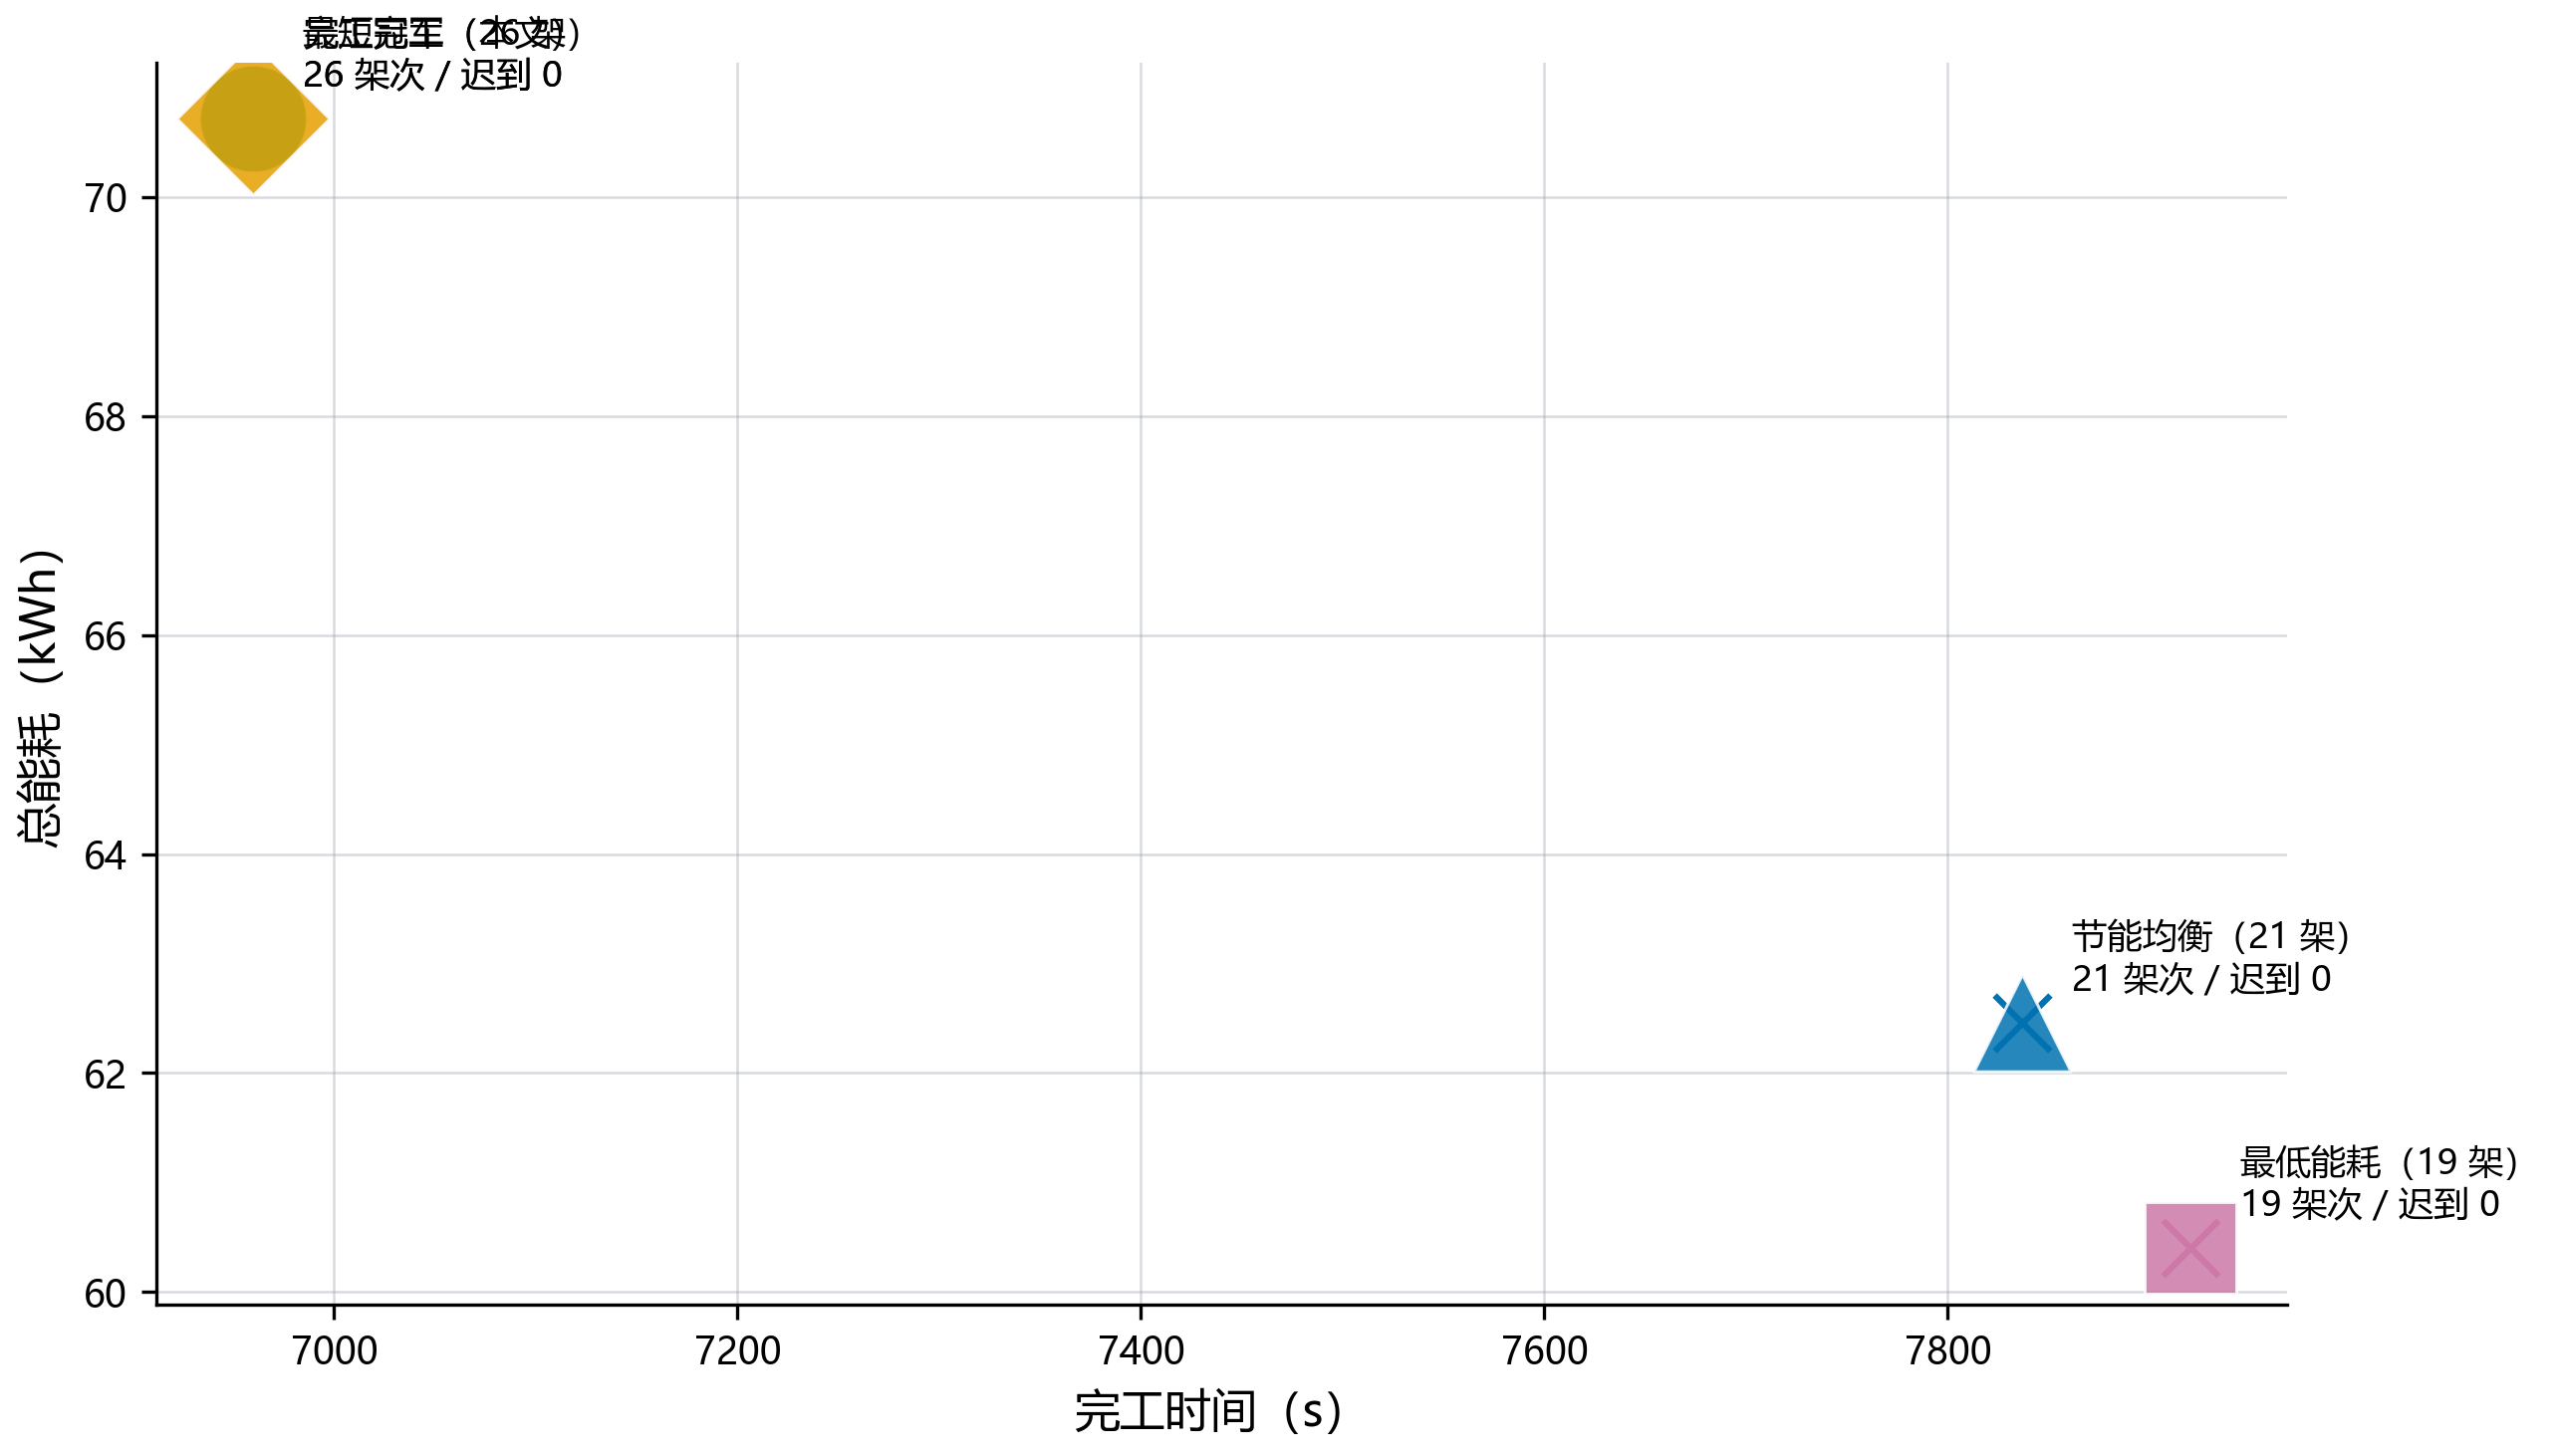
\includegraphics[width=0.86\textwidth]{figures/p2_pareto2d.png}
\caption{问题二多目标权衡（气泡大小为架次数）}
\label{fig:pareto2d}
\end{figure}

\subsubsection{均衡调度方案}

均衡方案共 26 架次，其中 A 型 12、B 型 7、C 型 7，全部 80 箱按时交付，即硬
约束满足且加权迟到为零，完工时间约 6960\,s，总能耗 70.71\,kWh。图
\ref{fig:p2net} 给出 26 架次在数字高程背景上的航线网络，可见 C 型航线构成
远距重载走廊，A、B 型负责短途轻载区；表 \ref{tab:p2flights} 给出架次明细，
图 \ref{fig:p2gantt} 给出各无人机的时间线，完整逐箱交付时刻见《结果提交
模板》Q2 工作表。

\begin{figure}[htbp]
\centering
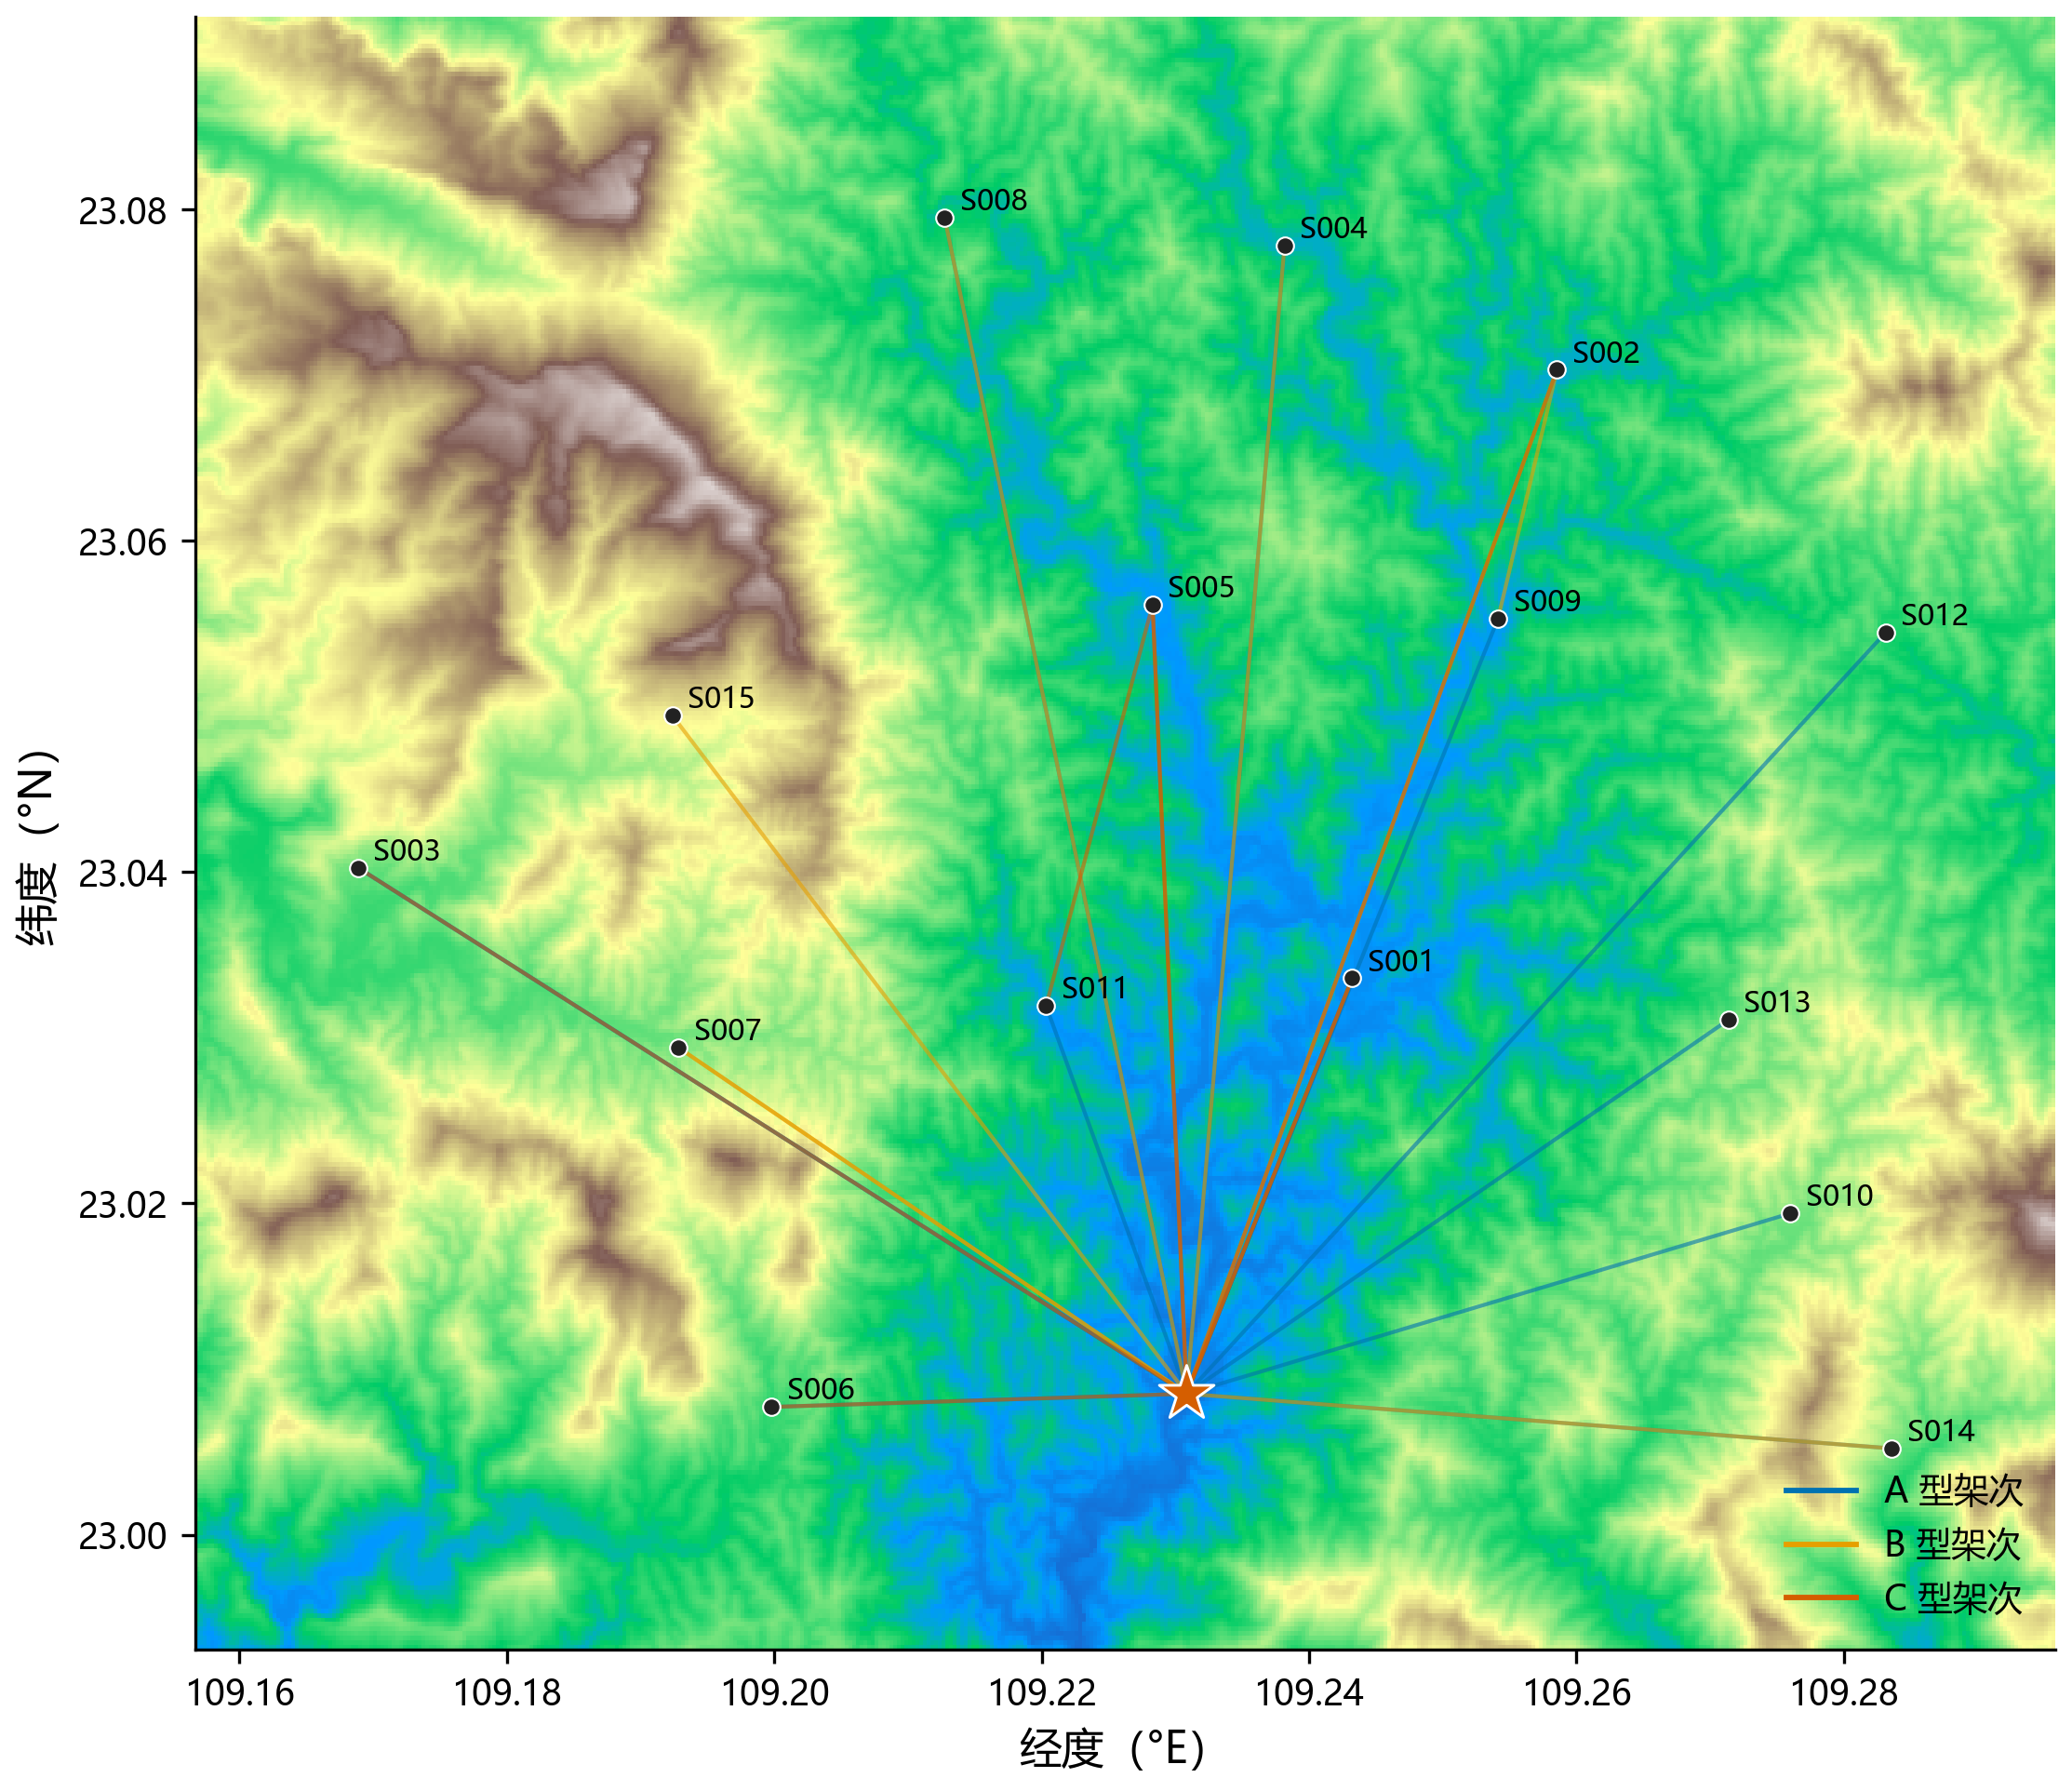
\includegraphics[width=0.82\textwidth]{figures/p2_network.png}
\caption{问题二均衡方案航线网络（按机型着色）}
\label{fig:p2net}
\end{figure}

\begin{table}[htbp]
\centering
\caption{问题二均衡调度方案（26 架次）}
\label{tab:p2flights}
\small
\begin{tabular}{ccccccc}
\toprule
架次 & 机型 & 无人机 & 开始(s) & 返回(s) & 能耗(kWh) & 航线 \\
\midrule
f24 & C & U08 & 0 & 1558 & 2.60 & S006 \\
f34 & C & U07 & 0 & 1559 & 2.99 & S001 \\
f18 & C & U08 & 1558 & 3595 & 5.52 & S002 \\
f17 & C & U07 & 1559 & 2986 & 2.40 & S001 \\
f23 & C & U07 & 2986 & 4926 & 4.39 & S005 \\
f20 & C & U08 & 3595 & 5949 & 5.46 & S003 \\
f05 & C & U07 & 4926 & 6960 & 3.81 & S005至S011 \\
\midrule
f07 & B & U06 & 0 & 1621 & 1.77 & S007 \\
f14 & B & U05 & 0 & 1861 & 1.99 & S014 \\
f35 & B & U06 & 1621 & 3182 & 1.69 & S007 \\
f02 & B & U05 & 1861 & 3825 & 2.63 & S002至S009 \\
f15 & B & U06 & 3182 & 5005 & 2.30 & S015 \\
f22 & B & U05 & 3825 & 5745 & 3.03 & S004 \\
f26 & B & U06 & 5005 & 6896 & 2.76 & S008 \\
\midrule
f01 & A & U01 & 0 & 1310 & 1.26 & S001 \\
f03 & A & U02 & 0 & 2310 & 3.03 & S003 \\
f06 & A & U03 & 0 & 1310 & 1.31 & S006 \\
f10 & A & U04 & 0 & 1649 & 1.95 & S010 \\
f12 & A & U01 & 1310 & 3357 & 2.91 & S012 \\
f04 & A & U03 & 1310 & 3487 & 3.08 & S004 \\
f31 & A & U04 & 1649 & 3255 & 1.94 & S013 \\
f32 & A & U02 & 2310 & 4291 & 2.27 & S014 \\
f21 & A & U04 & 3255 & 5505 & 3.08 & S003 \\
f08 & A & U01 & 3357 & 5458 & 3.14 & S008 \\
f09 & A & U03 & 3746 & 5432 & 2.25 & S009 \\
f11 & A & U02 & 4291 & 5507 & 1.15 & S011 \\
\bottomrule
\end{tabular}
\end{table}

\begin{figure}[htbp]
\centering
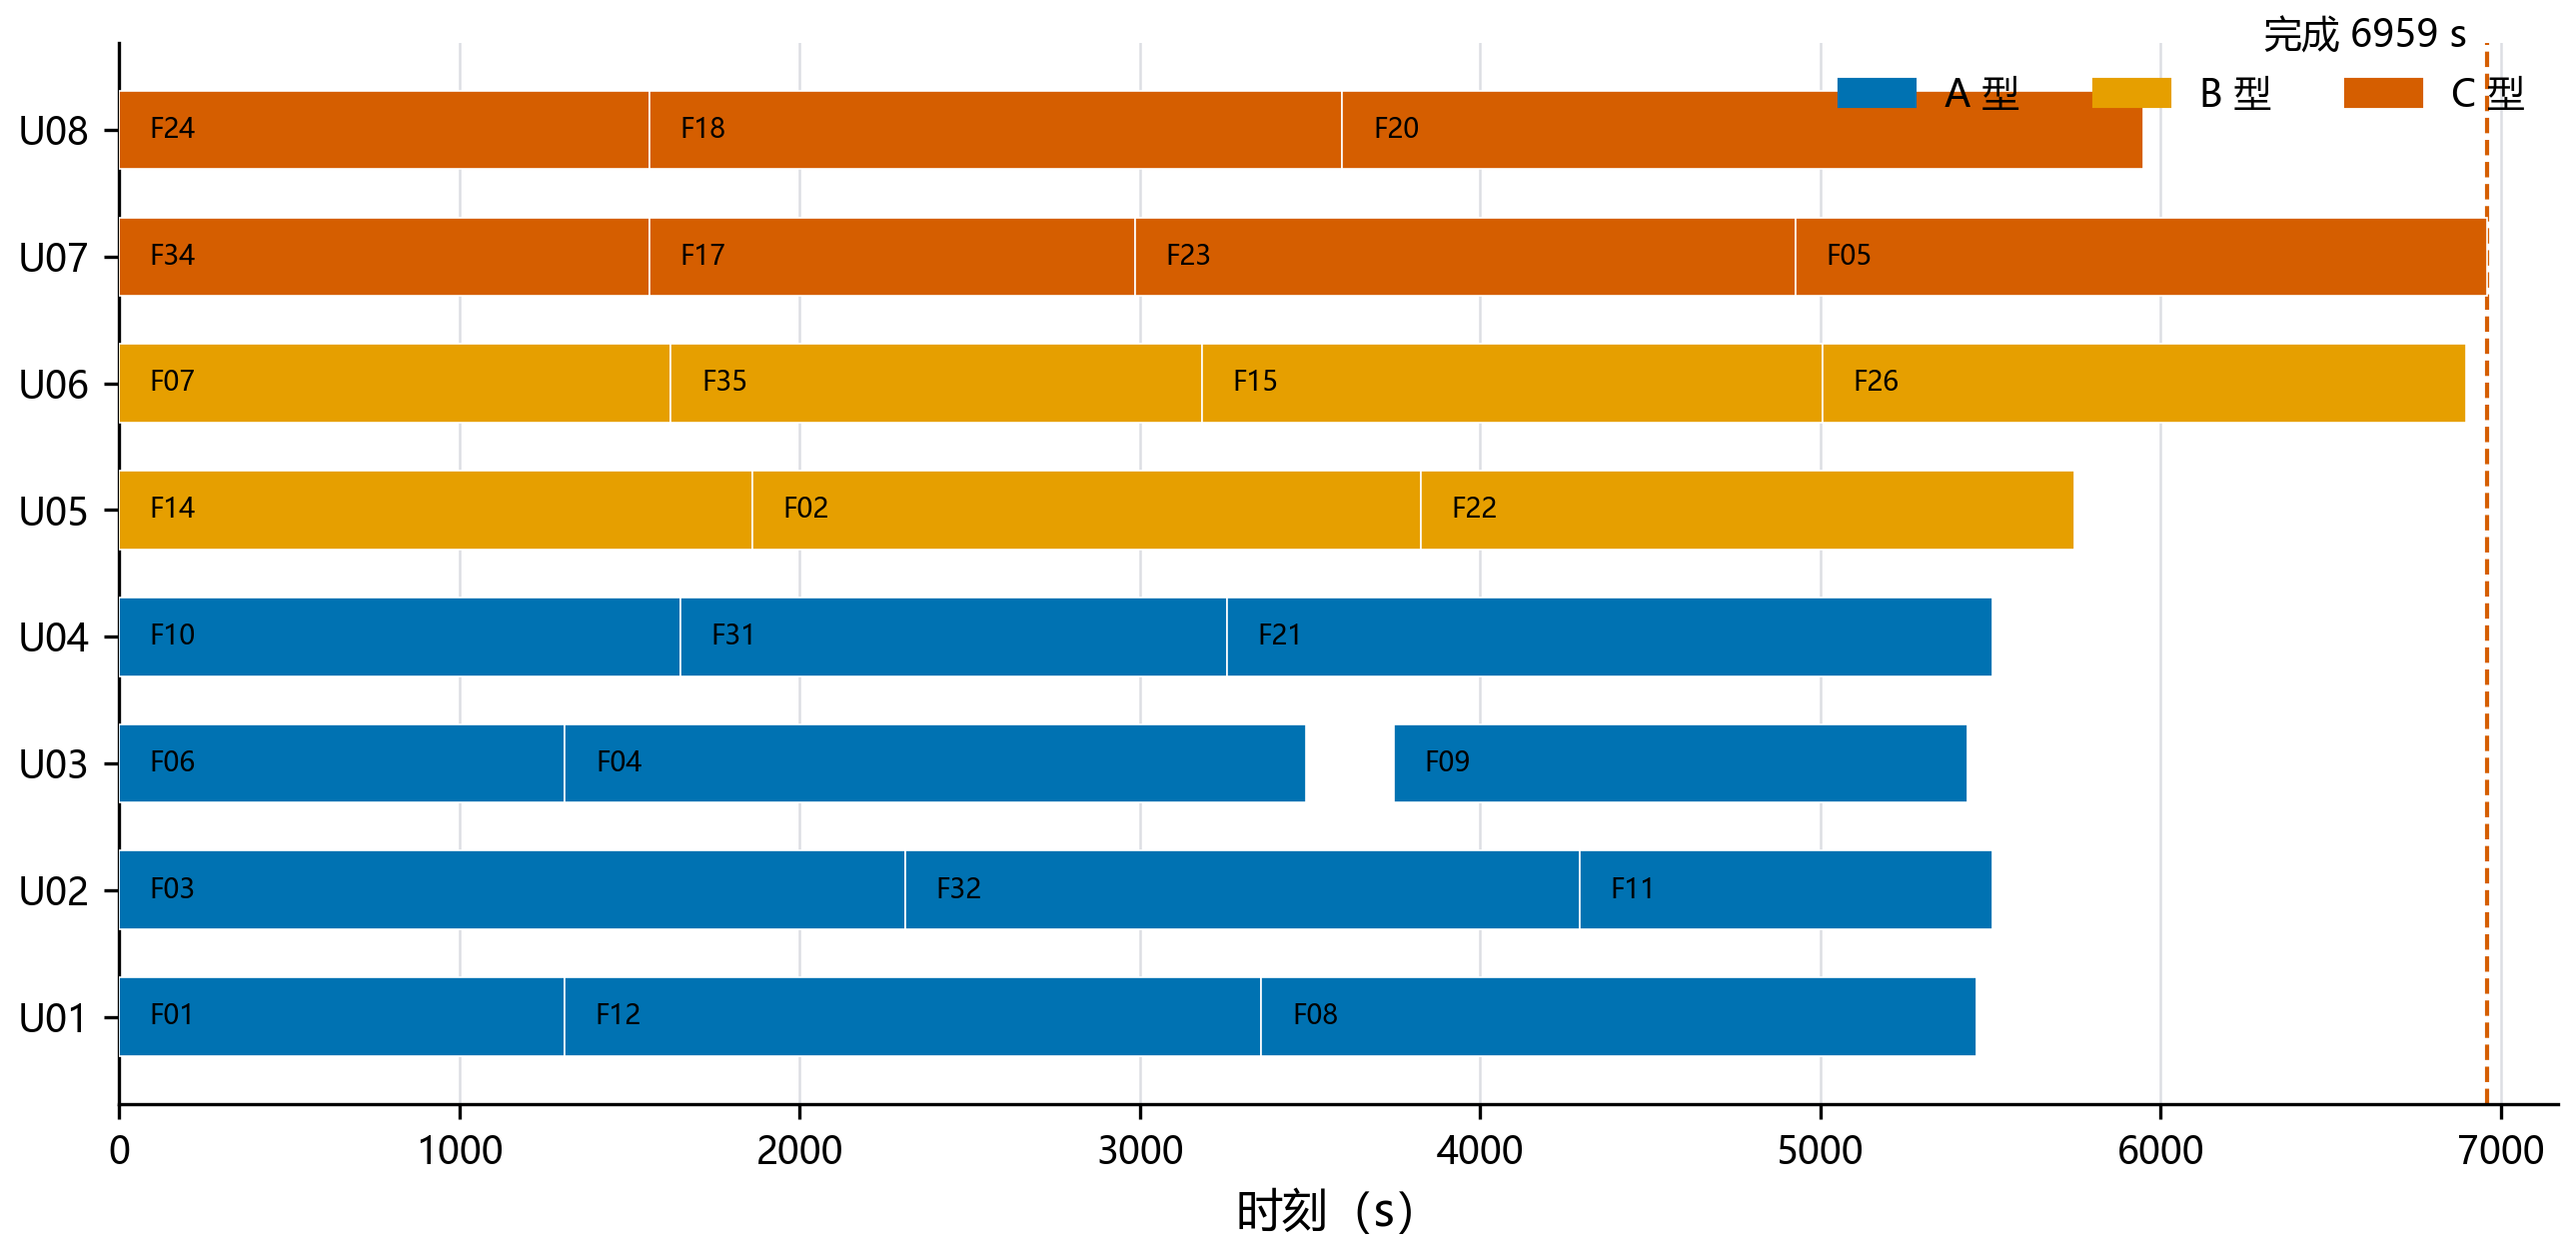
\includegraphics[width=0.95\textwidth]{figures/p2_gantt.png}
\caption{问题二均衡方案的运输任务甘特图（按无人机分泳道）}
\label{fig:p2gantt}
\end{figure}

\subsection{结果分析}

\begin{enumerate}
\item \textbf{C 型瓶颈}：7 个 C 架次承载了主要重载区任务，U07 与 U08 两架
C 型无人机几乎连续出勤至约 6960\,s，是完工时间的主要决定因素；A、B 型负责
轻载区与短途，链条明显更短，与远距重载只能由 C 型承担的物理规律一致。
\item \textbf{电池轮换充分}：共享电池在 26 架次中轮换，未出现电池短缺导致的
等待，说明电池数量不是瓶颈。图 \ref{fig:battery} 给出 14 组电池的任务段与
充电段时间线，充电按两阶段曲线，即低荷电快充后在 0.9 荷电以上转入慢充，使
电池在架次间隙即可恢复满电。

\begin{figure}[htbp]
\centering
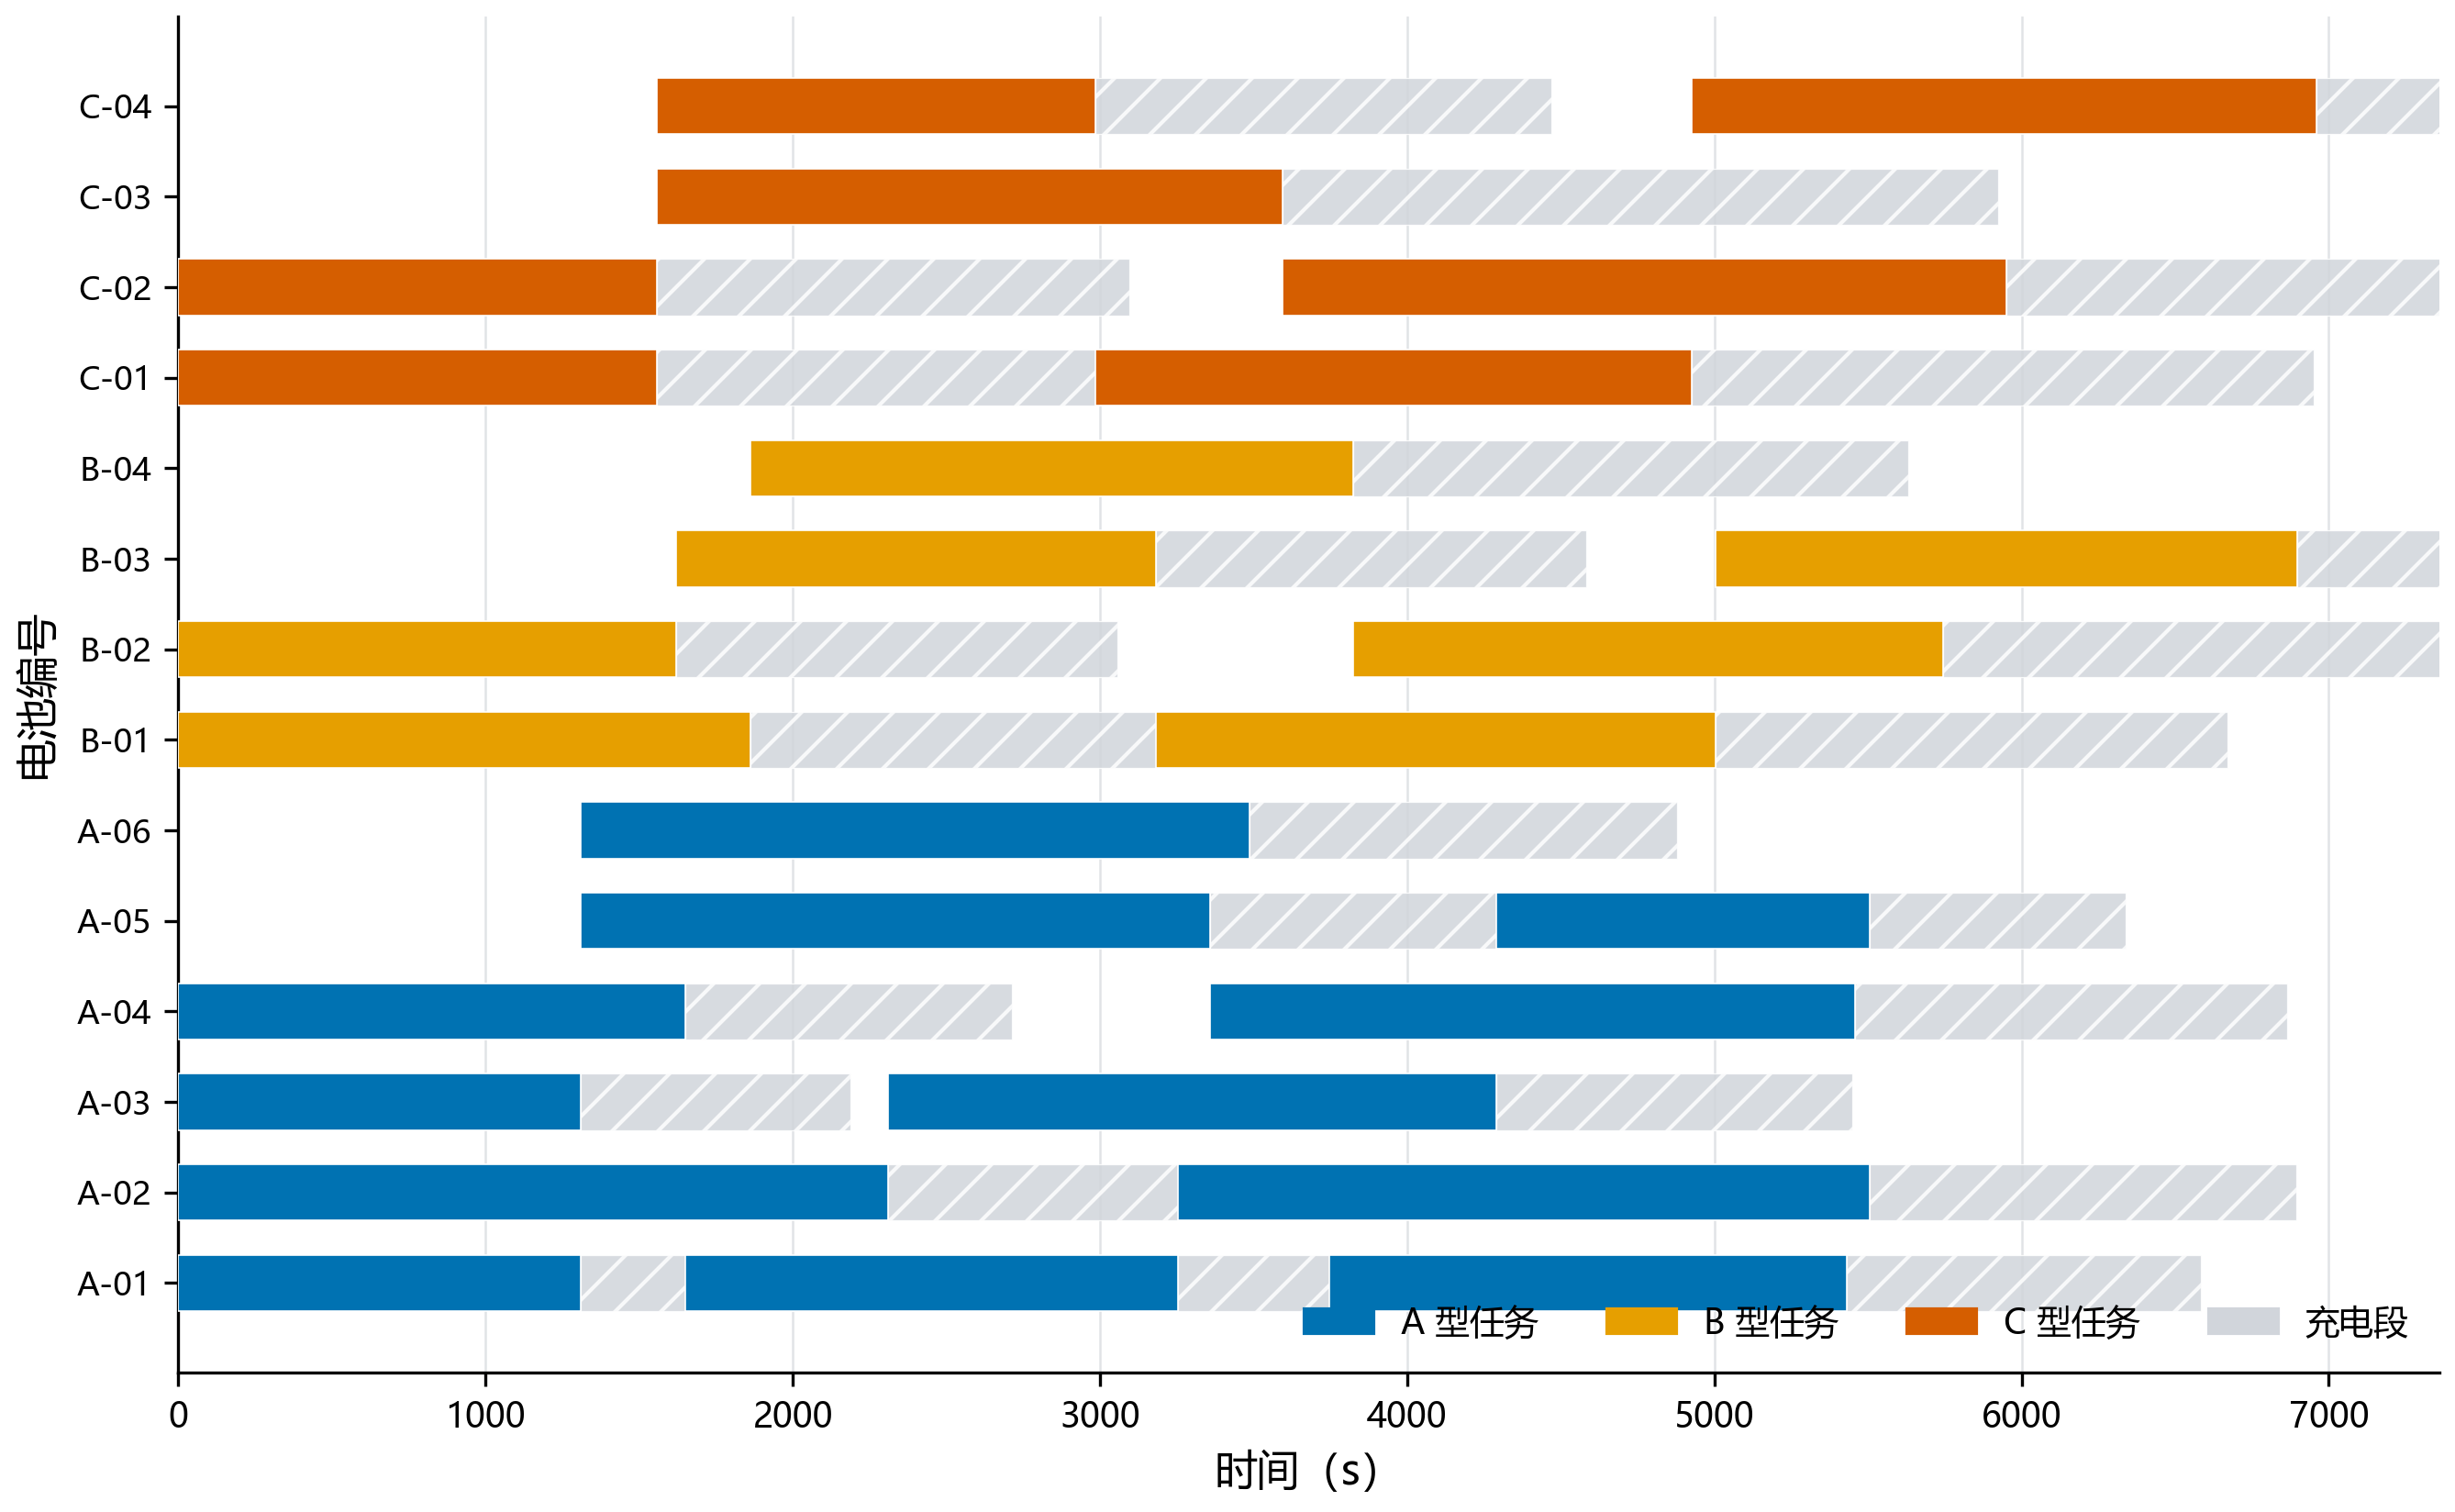
\includegraphics[width=0.98\textwidth]{figures/p2_battery.png}
\caption{14 组共享电池的任务与充电时间线（斜纹为充电段）}
\label{fig:battery}
\end{figure}

\item \textbf{时限全部满足}：首飞批货箱由首波架次优先送达，医疗货箱全部按
首飞批时限交付，普通批无超期。图 \ref{fig:delivery} 给出 80 箱的交付时刻与
配送时限散点，全部落在 45° 斜线以下，即交付不迟于时限；最紧裕度出现在
S004 服务区的最晚班次，系该区末班抵达所致。

\begin{figure}[htbp]
\centering
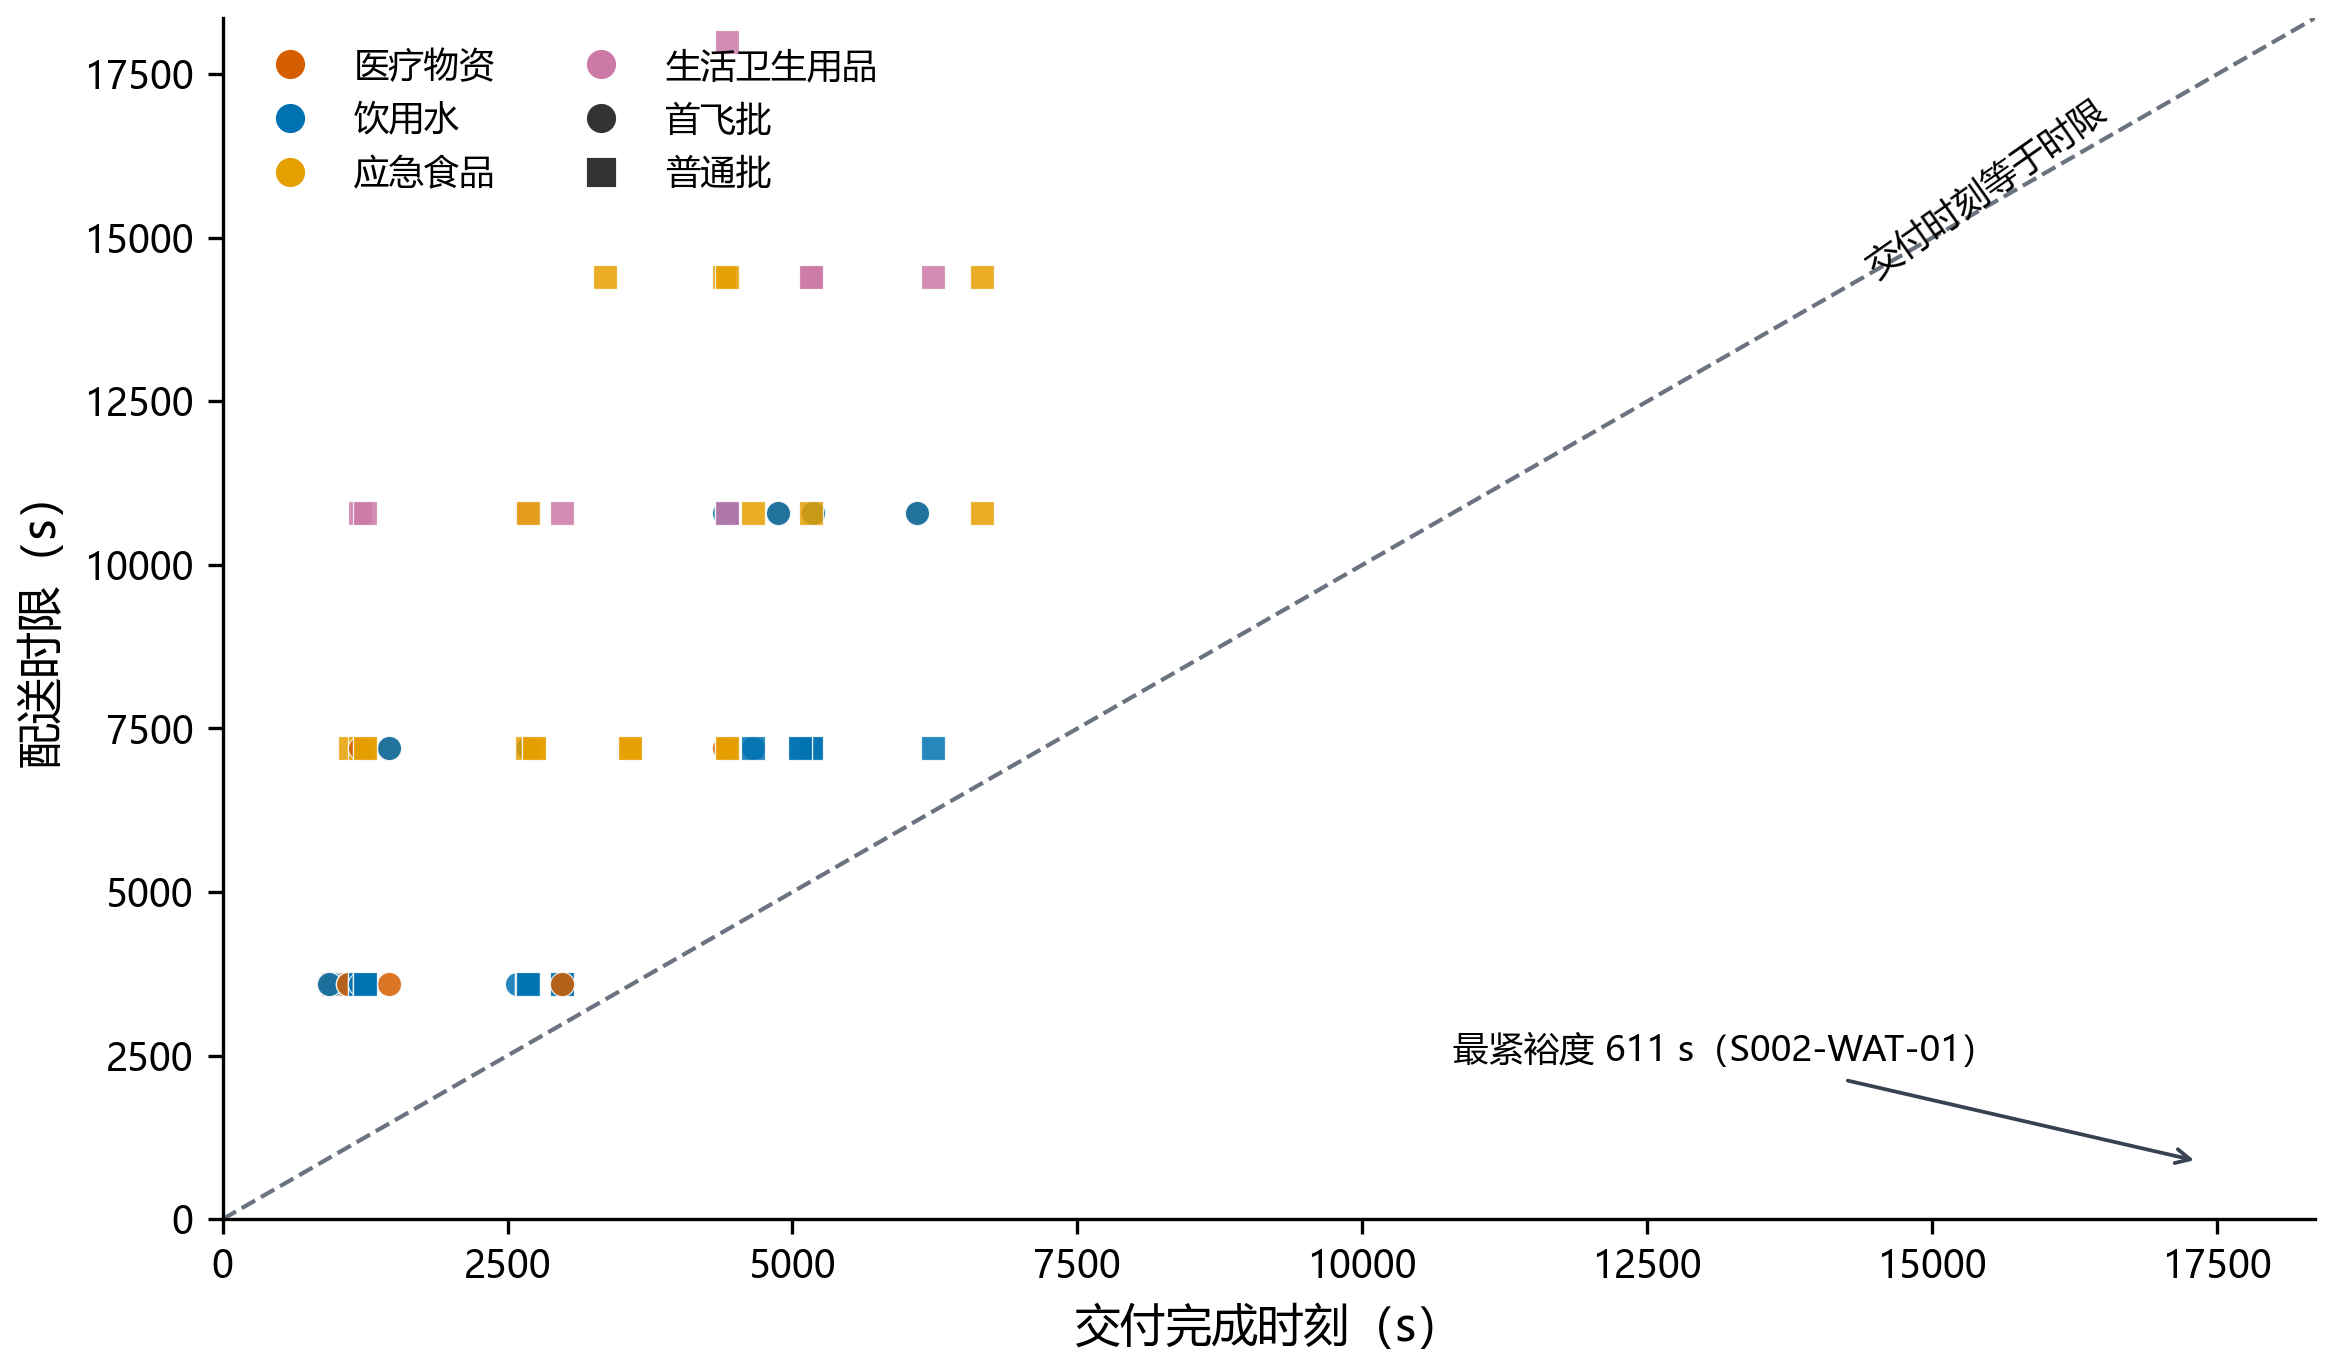
\includegraphics[width=0.86\textwidth]{figures/p2_delivery.png}
\caption{逐箱交付时刻与配送时限（圆点为首飞批，方块为普通批）}
\label{fig:delivery}
\end{figure}
\item \textbf{通信约束尚未计入}：本节的方案未考虑飞行全程通信，若按直连
判定，部分服务区作业段将被山体遮挡，需经中继保障，相关联合调度见第
\ref{sec:p3}节。
\end{enumerate}